\capitulo{5}{Aspectos relevantes del desarrollo del proyecto}

\section{Formación y aprendizaje necesario}

El desarrollo del proyecto requirió adquirir nuevos conocimientos y profundizar en diversas tecnologías y técnicas de análisis. A continuación, se describe la formación llevada a cabo en las herramientas y algoritmos más relevantes.

\subsection{Estudio del algoritmo TRACLUS}

El enfoque principal de este proyecto ha sido estudiar en profundidad el algoritmo \textbf{TRACLUS}, destinando una gran parte de las horas de investigación a comprender su funcionamiento y potencial para el análisis de trayectorias. Este algoritmo se basa en la segmentación y agrupación de trayectorias, permitiendo identificar sub-trayectorias comunes dentro de un conjunto de datos. Esto lo convierte en una herramienta valiosa para descubrir patrones significativos en datos de trayectorias. La investigación incluyó la revisión de artículos académicos y la exploración de cómo ajustar los parámetros de TRACLUS para maximizar su efectividad en el contexto específico del proyecto.

Adicionalmente, se evaluó el uso de una implementación de TRACLUS disponible en una biblioteca externa, explorando su viabilidad y características. Aunque esta versión fue útil para los primeros experimentos, se consideraron también posibles variantes y adaptaciones del algoritmo, con el fin de entender mejor el alcance y la adaptabilidad de TRACLUS.

Todos estos estudios fueron necesarios para cumplir con el objetivo del proyecto: implementar el algoritmo TRACLUS y compararlo con variantes del mismo, como las que se detallan a continuación.

\subsubsection{Propuesta de variantes de TRACLUS}

Durante el desarrollo del proyecto, se analizaron varias propuestas de variantes del algoritmo TRACLUS que han surgido en estudios recientes. Aunque finalmente no se utilizaron, debido al excesivo tiempo que llevaría desarrollar las nuevas variantes, la investigación detallada de estos derivados fue enriquecedora y ayudó a contrastar enfoques para una implementación eficiente. Las variantes de TRACLUS estudiadas fueron:

\begin{itemize}
    \item \textbf{GTraclus:} Una variante diseñada para ejecutarse en unidades de procesamiento gráfico (GPU), optimizando la eficiencia del algoritmo al aprovechar la capacidad de procesamiento paralelo de las GPUs \cite{gtraclus}.

    \item \textbf{ST-TRACLUS:} Esta versión incorpora una dimensión temporal además de la espacial, permitiendo realizar agrupamientos espaciotemporales de trayectorias, lo cual mejora la calidad del análisis para datos donde el tiempo es una variable relevante \cite{st-traclus}.

    \item \textbf{ND-TRACLUS:} Una extensión de TRACLUS que permite realizar el clustering en espacios de n dimensiones, expandiendo su aplicabilidad a trayectorias de mayor dimensionalidad \cite{nd-traclus}.

    \item \textbf{Neighborhood-Based Trajectory Clustering:} Una alternativa basada en densidad local de vecindad en lugar de densidad global. Este enfoque busca mantener la eficiencia de TRACLUS mientras reduce la necesidad de múltiples parámetros de entrada \cite{nb-traclus}.

    \item \textbf{Adaptive Trajectory Clustering based on Grid and Density (ATCGD):} Un método que introduce una cuadrícula y criterios de densidad para el análisis de patrones móviles, buscando reducir la complejidad computacional y la carga de trabajo en la calibración de parámetros, especialmente en aplicaciones a gran escala como la de trayectorias de vehículos en sistemas de transporte inteligente \cite{atcgd}.
\end{itemize}

\subsubsection{Variación de las técnicas de clustering}

Paralelamente a la investigación de las variantes de TRACLUS, se estudiaron técnicas adicionales de clustering, dado que el algoritmo requiere la clusterización de segmentos para su evaluación final. Con el objetivo de evaluar la viabilidad y robustez de TRACLUS, se analizaron diversas técnicas de clustering, y tras descartar varias por inviabilidad, se optó finalmente por emplear los siguientes algoritmos ya incluidos en la librería de \texttt{scikit-learn}:

\begin{itemize}
    \item \textbf{DBSCAN:} Algoritmo basado en densidad que identifica clusters de alta densidad separados por regiones de menor densidad, adecuado para datos espaciales y resistente al ruido.
    
    \item \textbf{OPTICS:} Similar a DBSCAN, pero permite una sensibilidad ajustable a la densidad, lo que lo hace más flexible para analizar datos con densidades variadas.

    \item \textbf{HDBSCAN:} Variante jerárquica de DBSCAN que ajusta automáticamente los parámetros de densidad, simplificando su aplicación en datos de densidad variable.

    \item \textbf{Spectral Clustering:} Algoritmo basado en el análisis de valores propios que es particularmente útil en datos no lineales o con clusters de formas complejas.

    \item \textbf{Agglomerative Clustering:} Método jerárquico ascendente que agrupa iterativamente elementos basándose en la proximidad, resultando útil en análisis donde la estructura jerárquica es relevante.
\end{itemize}

Cada técnica fue investigada en términos de sus características, sensibilidad a la densidad, capacidad de manejar ruido y aplicabilidad a datos espaciales. La exploración de estas técnicas permitió seleccionar aquellas que mejor se adaptaran a las necesidades específicas del proyecto y que complementaran el uso de TRACLUS en el análisis de trayectorias.

\subsection{Página Web}

El diseño de la página web comenzó con un prototipo básico que definía las funciones principales a implementar. La estructura inicial incluía:  
\begin{itemize}
    \item Una página para visualizar los datos sin procesar en forma de mapas de trayectorias y mapas de calor.
    
    \begin{figure}[h!]
    		\centering
    		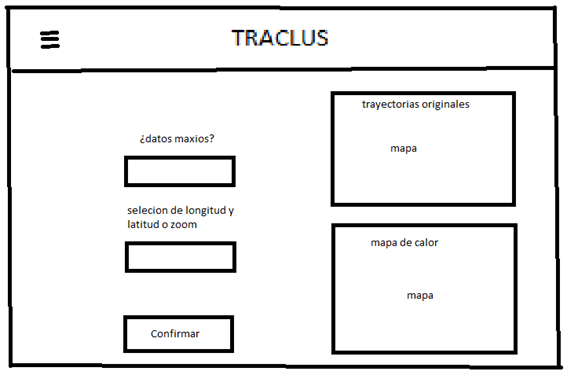
\includegraphics[width=0.5\textwidth]{img/prototipo_web1.png}
    		\caption{Código innecesario.}
	\end{figure}
	\FloatBarrier
    
    \item Una segunda página dedicada a la comparativa de \textit{clusters} mediante mapas interactivos.
    
    \begin{figure}[h!]
    		\centering
    		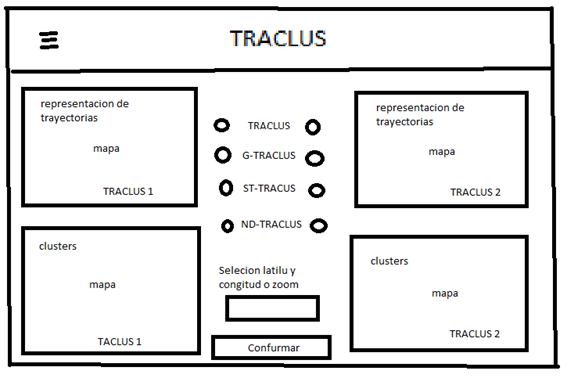
\includegraphics[width=0.5\textwidth]{img/prototipo_web2.png}
    		\caption{Código innecesario.}
	\end{figure}
	\FloatBarrier
    
    \item Una tercera página para analizar la relación entre trayectorias y \textit{clusters} generados por diferentes algoritmos.
    
    \begin{figure}[h!]
    		\centering
    		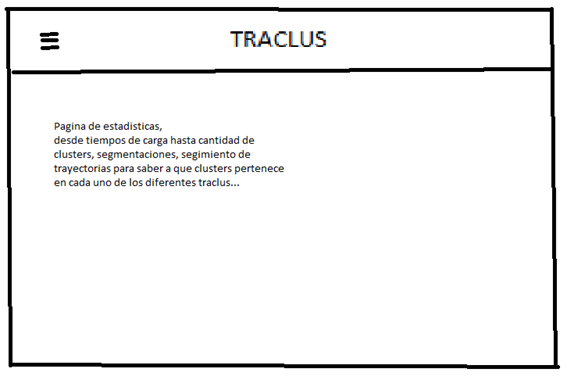
\includegraphics[width=0.5\textwidth]{img/prototipo_web3.png}
    		\caption{Código innecesario.}
	\end{figure}
	\FloatBarrier
\end{itemize}

El desarrollo requirió integrar la biblioteca Dash con herramientas adicionales como \texttt{CSS Grid} para gestionar el diseño de los componentes. Para optimizar tiempos de carga, se decidió prerenderizar imágenes y tablas, limitando las opciones disponibles a configuraciones predefinidas.

Durante el proyecto, el diseño evolucionó para mejorar la experiencia del usuario. La página inicial se dividió en dos: una para la carga de datos y otra para la visualización de trayectorias. Además, se añadieron nuevas funcionalidades, como un botón para descargar datos generados y pantallas adicionales que permitían seleccionar algoritmos de \textit{clustering} o reutilizar experimentos previos.

El menú desplegable inicial fue sustituido por una barra de navegación, lo que simplificó la interacción entre las diferentes páginas. También se eliminaron características que no aportaban valor significativo, como el zoom en los mapas, y se adoptó un enfoque basado en el modelo vista-controlador para estructurar el proyecto de manera más eficiente.

\section{Optimización}

El que podríamos considerar como el segundo punto más relevante, y sin duda uno de los aspectos críticos del proyecto, han sido los tiempos de ejecución. Debido a las grandes cantidades de datos a procesar, cada cálculo y visualización requerían una considerable cantidad de tiempo, por lo que la optimización de tiempos se convirtió en una prioridad clave para asegurar la viabilidad del proyecto.

\subsection{Visualización y dibujado de Mapas}

El primer desafió en el rendimiento fue la visualización de mapas, especialmente al intentar realizar representaciones detalladas y visualmente atractivas. Al analizar distintas bibliotecas de Python para dibujar y visualizar mapas, se probaron y compararon múltiples opciones combinadas entre si, como \texttt{pandas}, \texttt{geopandas}, \texttt{folium}, \texttt{folium.plugins}, \texttt{matplotlib.pyplot}, \texttt{matplotlib.colors}, \texttt{contextily}, \texttt{pyproj}, \texttt{seaborn}, \texttt{pydeck}, \texttt{shapely.geometry}, \texttt{sklearn.preprocessing} y \texttt{scipy.stats}.

Tras diversas pruebas de rendimiento y calidad visual, se optó por utilizar principalmente \texttt{contextily} y \texttt{matplotlib.pyplot} para la visualización de mapas, ya que estas bibliotecas ofrecieron la mejor relación entre rendimiento y calidad gráfica. Para la visualización de \textit{heatmaps}, se incluyeron \texttt{numpy} como las opciones más eficientes para generar mapas de calor. Sin embargo, para lograr un equilibrio óptimo entre rendimiento y visualización, se sacrificaron ciertas funcionalidades como el zoom en mapas interactivos y detalles visuales avanzados.


\subsection{Optimización del algoritmo}

Uno de los principales desafíos del proyecto fue el tiempo de procesamiento, debido a la gran cantidad de datos que debían manejarse. El tamaño y la complejidad de los datos afectaron tanto la carga inicial como la ejecución de algoritmos y la visualización, requiriendo una optimización constante para lograr resultados en tiempos razonables.

\subsubsection{Carga de Datos}

El primer obstáculo en términos de tiempo fue la carga de datos en la aplicación web, ya que \texttt{Dash} tiene limitaciones al cargar grandes volúmenes de datos. El archivo inicial pesaba aproximadamente dos gigabytes, y ni siquiera herramientas como Excel podían manejar correctamente un CSV de este tamaño, lo que llevó a errores frecuentes al intentar reducir su tamaño sin comprometer la integridad de los datos.

Tras varios intentos de conversión y reducción, se logró un tamaño adecuado que permitió cargar los datos en la aplicación. Además, para estructurar y analizar los datos en trayectorias geográficas, fue necesario procesarlos con \texttt{GeoDataFrame} mediante la biblioteca \texttt{GeoPandas}. Gracias a esta biblioteca, el tiempo de carga y procesamiento fue moderado y permitió manipular los datos de forma eficiente para futuras visualizaciones y análisis.

Para la visualización, el tamaño del conjunto de datos impactó en la calidad gráfica y los tiempos de carga. Fue necesario optar por bibliotecas de visualización que equilibraran la calidad y el tiempo de renderizado, sacrificando algunas características visuales avanzadas en favor de un rendimiento adecuado. Finalmente, se optó por \texttt{contextily} y \texttt{matplotlib.pyplot} para la representación de mapas y \texttt{numpy} para los mapas de calor.

\subsubsection{Distancias}

El proceso más complejo y exigente en términos de tiempo fue la ejecución del algoritmo TRACLUS. Durante su ejecución, es necesario calcular las distancias perpendicular, paralela y angular entre todas las trayectorias, lo que genera una complejidad algorítmica exponencial \(O(n^2)\). Esto se vuelve aún más costoso cuando se desean evaluar varias opciones de clustering en el mismo conjunto de datos.

Antes de las optimizaciones, el programa tardaba aproximadamente dos minutos y cuarenta y cinco segundos en cargar cien filas de datos, y una hora y cinco minutos en cargar quinientas filas, lo cual era insostenible dado que el archivo fuente de datos del proyecto contenía más de un millón de filas.

Para reducir estos tiempos, se realizaron múltiples pruebas y técnicas de optimización:

\begin{enumerate}
    \item \textbf{Numpy para la matriz de distancia:} Inicialmente, se intentó cargar la matriz de distancia utilizando \texttt{numpy}, que es una biblioteca altamente optimizada para cálculos matemáticos. Sin embargo, los resultados generados no coincidían con los obtenidos mediante el cálculo original, lo que condujo a diferencias significativas en los resultados de clustering.

    \item \textbf{Vectorización con Numpy:} En un segundo intento, se volvió a probar con \texttt{numpy}, aplicando un enfoque más completo de vectorización para las tres distancias. Nuevamente, aunque los tiempos de ejecución mejoraron, los resultados no fueron precisos, afectando la coherencia en los datos obtenidos.

    \item \textbf{Threading con bucles:} Para el tercer intento, se reutilizaron las funciones originales de cálculo de distancias, pero paralelizando los tres bucles de cálculo de distancias mediante \texttt{threading}. Esta prueba mejoró los tiempos levemente, reduciendo la carga de cien filas a dos minutos y veintidós segundos, manteniendo los resultados consistentes, aunque la mejora fue insuficiente para los objetivos del proyecto.

    \item \textbf{ThreadPoolExecutor y chunks:} En la cuarta prueba, se dividió la matriz de distancia en “chunks” para ser procesados en paralelo con \texttt{ThreadPoolExecutor}. Sin embargo, esta técnica solo generó una mejora marginal, con una reducción de aproximadamente seis segundos en la carga de cien filas, lo cual, aunque significativo para cantidades de datos pequeñas, resultó ineficiente para volúmenes mayores.

    \item \textbf{Paralelización manual y threading:} Finalmente, se probó una combinación de threading, sin usar \texttt{numpy} para los cambios en las funciones de distancia, calculando las distancias en tres hilos independientes. Este enfoque proporcionó el mejor resultado, logrando una reducción de tiempo a la mitad: un minuto y cuatro segundos para cien filas, y treinta y un minutos y cuarenta y nueve segundos para quinientas filas. Sin embargo, aunque esta reducción era significativa, los tiempos seguían siendo elevados para la totalidad de los datos del proyecto.
\end{enumerate}

Este proceso de optimización requirió numerosos ajustes y pruebas incrementales, en muchos casos con cambios mínimos y variaciones en el tamaño de los datos de prueba, lo que demandó una gran cantidad de horas de prueba y error sin obtener los resultados esperados. No se tiene un cálculo exacto, pero este apartado del proyecto consumió no solo decenas, sino cientos de horas dedicadas exclusivamente a la ejecución y análisis de pruebas.

En conclusión, aunque Python es un lenguaje versátil, sus limitaciones en paralelización y threading efectivo complicaron la optimización de cálculos intensivos en comparación con otros lenguajes como Java, lo que limitó el rendimiento alcanzable en este proyecto.


\subsection{Optimización de la página web} 

Tras múltiples ejecuciones de la página web para comparar los resultados de los diferentes algoritmos de clustering aplicados al TRACLUS, se identificó un problema recurrente: el tiempo de ejecución elevado.

En la aplicación, se podían ejecutar hasta cinco veces consecutivas el algoritmo TRACLUS, cada vez con modificaciones en el algoritmo de clustering. Esta ejecución lineal incrementaba significativamente los tiempos, ya que incluso con pocos datos, el algoritmo mostraba lentitud.

\subsubsection{Estrategia inicial: Uso de hilos}
Para abordar este problema, se reutilizó una estrategia previamente implementada: el uso de hilos. En el controlador \texttt{clustering.py}, que ya gestionaba correctamente el flujo de carga de datos, se dividió el código en funciones separadas, una por cada algoritmo de clustering. Estas funciones eran llamadas según las selecciones del usuario mediante la biblioteca \texttt{threading}.

\subsubsection{Problemas con la generación de mapas y tablas}
Posteriormente, se intentó incorporar la creación de mapas y tablas a estos hilos. Sin embargo, surgieron incompatibilidades con la biblioteca \texttt{matplotlib}, que no es compatible con librerías de hilos como \texttt{concurrent-} \texttt{.futures} o \texttt{threading}. Por este motivo, se decidió separar estas tareas. Una vez finalizados todos los hilos, se invocaba una nueva función encargada de generar los mapas necesarios para visualizar los datos.

\subsubsection{Limitaciones de Python}
Aunque esta optimización redujo el tiempo de ejecución, los resultados no alcanzaron las expectativas iniciales. Se identificó que la principal limitación era Python. Su configuración interna impide utilizar múltiples núcleos del procesador de manera eficiente, lo que restringía la velocidad máxima en dispositivos locales. Sin embargo, estas limitaciones no afectaban significativamente la aplicación en entornos remotos, donde el alto rendimiento no era una prioridad debido a los costes asociados.

\subsubsection{Exploración de alternativas de paralelización}
Dado el potencial escalamiento de la aplicación, se exploraron otras estrategias de paralelización:
- \texttt{asyncio}: Diseñada para tareas intensivas en I/O, pero no adecuada para este caso.
- \texttt{Batch Processing}: Orientada a flujos simples, tampoco era aplicable.
- \texttt{Dask} y \texttt{ProcessPoolExecutor}: Ambas opciones cumplían con los requisitos del proyecto.

Se optó por \texttt{ProcessPoolExecutor} debido a su menor complejidad y capacidad para ejecutar funciones en diferentes núcleos del procesador.

\subsubsection{Optimización del flujo de datos}
Además del uso de \texttt{multiprocessing}, se unificó el flujo de representación de los datos en las funciones de multiproceso, lo que resolvió incompatibilidades previas con \texttt{matplotlib}. Esto incrementó considerablemente el rendimiento, ya que anteriormente estas tareas se ejecutaban en serie.

\subsubsection{Resultados obtenidos}
Tras implementar estas mejoras, se lograron resultados significativos:
- \textbf{Operaciones singulares}: La ejecución de un solo TRACLUS con 100 filas de datos pasó de 312 segundos a 288 segundos.
- \textbf{Ejecuciones simultáneas}: La ejecución de cinco TRACLUS con sus respectivos algoritmos de clustering se redujo drásticamente, de 1800 segundos a 450 segundos.

Esta optimización no solo mejoró el rendimiento, sino que también eliminó errores previamente asociados al uso de hilos.


\section{Testing}

Para que un código sea verdaderamente funcional, seguro y mantenible, debe someterse a pruebas exhaustivas. Durante el desarrollo del proyecto, se implementaron varios tipos de pruebas para evaluar el rendimiento y la calidad del código, así como para ampliar el conocimiento en el campo del testing.

\subsection{Análisis de código estático}

El análisis de código estático es una técnica utilizada para identificar posibles errores en el código fuente sin necesidad de ejecutarlo. Este método es particularmente útil para evitar fallos humanos como bucles infinitos, errores de formato o problemas de nomenclatura.

Se evaluaron varias herramientas de análisis estático teniendo en cuenta las siguientes limitaciones:
\begin{itemize}
    \item Debían ser compatibles con Python y CSS, los lenguajes utilizados en el proyecto.
    \item No debían implicar costos adicionales.
    \item Era deseable la integración directa con GitHub para facilitar el flujo de trabajo.
\end{itemize}

Con estas características, se seleccionaron dos herramientas principales: \textbf{SonarQube} y \textbf{Code Climate}. De estas, \textbf{SonarQube} fue la más utilizada, ya que ofrecía soporte para analizar IPython Notebooks, un formato clave en los experimentos realizados durante el proyecto. Aunque los notebooks no formaban parte directa de la aplicación web, su análisis fue crucial para garantizar la calidad de los experimentos previos.

Lo ideal en este tipo de análisis es aplicarlo de manera continua durante las diversas fases del proyecto, ya que esto reduce significativamente la carga de trabajo y mejora la calidad del código a medida que se desarrolla. Sin embargo, en este proyecto, el análisis estático se realizó al final, lo que no fue óptimo pero permitió identificar una serie de problemas, entre ellos:

\begin{itemize}
    \item \textbf{Mejoras en nomenclatura:} Se ajustaron nombres de variables para facilitar su comprensión y evitar confusiones con otros datos.
    
\begin{figure}[h!]
    \centering
    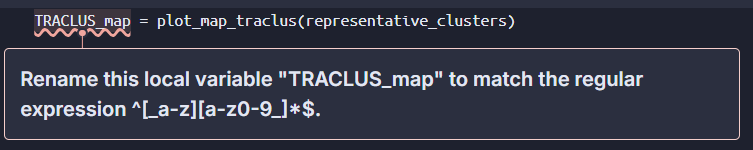
\includegraphics[width=0.5\textwidth]{img/sonarq_regularexp.png}
    \caption{Error nomenclatura.}
    \label{fig:trayectorias_Spectral}
\end{figure}    
    
    \item \textbf{Variables no utilizadas:} Se detectaron y eliminaron variables que ya no eran relevantes, ya fuera por errores en su definición o por haber quedado obsoletas durante el desarrollo.
    
\begin{figure}[h!]
    \centering
    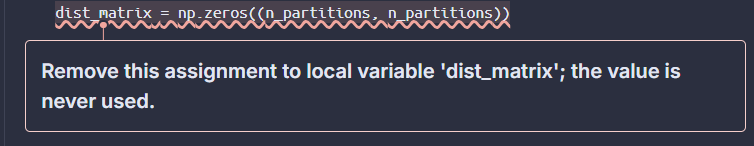
\includegraphics[width=0.5\textwidth]{img/sonarq_codigo_sobrante.png}
    \caption{Código innecesario.}
    \label{fig:trayectorias_Spectral}
\end{figure}

\begin{figure}[h!]
    \centering
    
\includegraphics[width=0.5\textwidth]{img/sonarq_unused.png}
    \caption{Variable sin usar necesaria.}
    \label{fig:trayectorias_Spectral}
\end{figure}    
    
    \item \textbf{Importaciones innecesarias:} Se eliminaron módulos y librerías no utilizadas, lo que ayudó a reducir la carga del programa y mejorar su legibilidad.
    
\begin{figure}[h!]
    \centering
    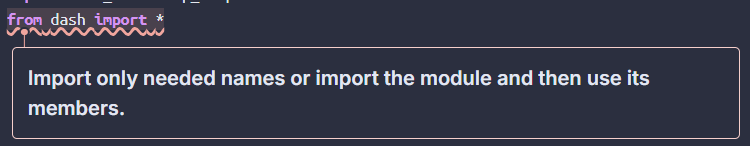
\includegraphics[width=0.5\textwidth]{img/sonarq_imports.png}
    \caption{Importación excesiva.}
    \label{fig:trayectorias_Spectral}
\end{figure}
   
    \item \textbf{Complejidad en funciones:} Se identificaron funciones cuya complejidad excedía los límites recomendados. Aunque algunas de estas funciones no pudieron simplificarse debido a las características del algoritmo, el análisis ayudó a priorizar futuras mejoras.
    
\begin{figure}[h!]
    \centering
    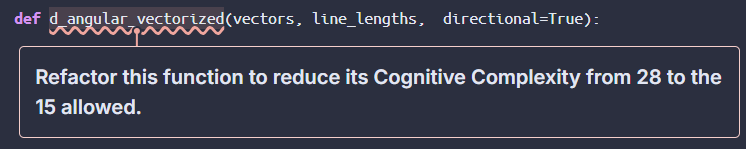
\includegraphics[width=0.5\textwidth]{img/sonarq_complex.png}
    \caption{Complejidad grande.}
    \label{fig:trayectorias_Spectral}
\end{figure}

\end{itemize}

Aunque este tipo de análisis no corrige directamente errores en la funcionalidad del algoritmo, resulta muy útil para evitar problemas menores, mejorar la mantenibilidad del código y garantizar un nivel básico de seguridad.

\subsection{Pruebas unitarias y su implementación}

Las pruebas unitarias son fundamentales para garantizar la funcionalidad de cada componente del código y asegurar que los resultados generados sean consistentes y correctos. Durante el desarrollo de la aplicación, se planteó inicialmente realizar pruebas unitarias utilizando \texttt{pytest} que evaluaran el comportamiento de cada botón y función de la aplicación mientras esta se ejecutaba. El objetivo era cubrir todo el flujo de la web en tiempo real, desde la interacción del usuario con los botones hasta la ejecución de los \texttt{callbacks} de Dash.

Sin embargo, esta aproximación presentó múltiples problemas. Dash, como framework basado en componentes interactivos, no es directamente compatible con las herramientas de testing tradicionales. Intentar realizar pruebas unitarias mientras la aplicación se encontraba en ejecución resultó inviable, ya que las pruebas no se ejecutaban correctamente, y la interacción con los componentes de la interfaz gráfica no podía ser simulada adecuadamente. Como resultado, las pruebas terminaban siendo llamadas directas a las funciones asociadas a los botones, sin representar el comportamiento real del flujo de la aplicación ni garantizar que los \texttt{callbacks} funcionaran en contexto.

Ante esta limitación, se decidió cambiar el enfoque hacia pruebas más efectivas y relevantes. La nueva estrategia consistió en lo siguiente:

\begin{itemize}
    \item \textbf{Pruebas de funciones críticas:} Se probaron de manera individual las funciones más importantes de los modelos, como la implementación del algoritmo TRACLUS y su integración con diferentes algoritmos de clustering. Estas pruebas se realizaron utilizando conjuntos de datos generados de manera aleatoria para garantizar que el comportamiento del código fuese robusto ante diferentes escenarios.
    \item \textbf{Representación de mapas:} Se verificó que las funciones encargadas de generar mapas, tanto de segmentos como de clústeres, produjeran respuestas correctas. 
\end{itemize}









